\documentclass[12]{article}
\usepackage{titlesec}
\usepackage{indentfirst}
\usepackage [french]{babel}
\usepackage [utf8]{inputenc}
\usepackage [T1] {fontenc}
\usepackage{subfiles}
\usepackage{wrapfig}
\usepackage{graphicx}
\usepackage{sidecap}
\usepackage{amssymb}
\usepackage{amsmath}
\usepackage{multirow}
\usepackage[french]{babel}
\graphicspath{ {./images/} }
\usepackage[export]{adjustbox}
\usepackage{enumitem}
\usepackage[absolute,overlay]{textpos}
\usepackage{float}
\usepackage{forest}
\usepackage{amsmath,amsfonts,amsthm,amssymb}
\usepackage{graphicx}
\usepackage{pdfpages}
\usepackage{amsmath}
\addtocontents{toc}{\protect\thispagestyle{empty}}
\usepackage[margin = 2.8 cm, headheight = 1.5pt]{geometry}
\usepackage{hyperref}
\usepackage{graphicx}
\usepackage{siunitx}

\usepackage{colortbl}
\usepackage{textgreek}



\begin{document}


\begin{titlepage}
\includepdf[fitpaper]{title}
\end{titlepage}

\newpage
\tableofcontents
\listoffigures
\newpage
\clearpage
\setcounter{page}{1}


\section*{Introduction - Paul Morel} 
Dans le cadre de notre projet APP, nous relevons le défi lancé par Events IT. Dans ce rapport notre mission est d’explorer et identifier les technologies de télécommunication les plus performantes spécifiquement adaptées à nos festivals. L'objectif est clair : garantir que nos capteurs communiquent via le canal le plus efficace possible. \\

Dans ce rapport, nous analysons l'usage des technologies de communication de pointe pour améliorer l'ambiance sonore des événements musicaux en extérieur. Nous prenons en compte la santé auditive des participants notamment grâce à un feedback en direct qui sera fait sur le site via l'interface utilisateur. En s'appuyant sur une analyse approfondie des spécifications techniques des différents moyens de communication telles que le Bluetooth, le Wi-Fi, la 4G, et la fibre optique. Le but est de mettre en place un système fiable et performant pour la collecte, le traitement et la diffusion des données sur le niveau sonore, assurant ainsi une expérience sûre et enrichissante pour les utilisateurs et pour l'organisateur. Ce document vise à établir un dialogue constructif entre la technologie, le bien-être et l'innovation. \\

L'adoption de ces technologies de communication dans notre initiative va au-delà du simple échange de données. Elle est partie intégrante d'une vision plus importante qui cherche à rehausser le bien-être des utilisateurs tout en rendant l'organisation et la gestion d'événements musicaux (festivals) plus efficaces. Avec une attention particulière portée à la santé des utilisateurs / spectateurs, notre solution se positionne comme une innovation clé pour développer des espaces sonores à la fois sécuritaires et plaisants. Cette stratégie englobe non seulement un avantage pour les participants, en les informant sur les risques liés à l'exposition sonore, mais elle est aussi précieuse pour les organisateurs. Ils disposent désormais d'un moyen efficace pour surveiller et ajuster le volume sonore, garantissant une qualité d'expérience musicale plaisante. \\


\section{Spécifications des réseaux sans fil}

\subsection{Spécifications du Bluetooth - Romain Oualid}

La société Events-IT nous a donné pour mission l'analyse d'un transfert de fichier via Bluetooth entre deux équipements. D'un côté, un smartphone (objet) qui joue le rôle de récepteur et de l'autre un PC portable (passerelle) qui est l'émetteur. 

Nous savons que l'entreprise qui nous a communiqué notre mission souhaite déployer 35 objets sur une surface de 400 m². En revanche, une passerelle ne peut pas gérer une infinité d'objets simultanément. Après documentation, nous avons confirmé que la passerelle pouvait gérer 7 objets au maximum, il y a donc 1 maître (passerelle) pour 7 esclaves actifs (objets). Pour conclure, partons du principe que les 35 objets sont actifs en simultanée, il faudra donc 5 maîtres qui géreront chacun 7 esclaves. 

\subsection{Spécifications du Wi-Fi - Romain Oualid}

Le Wi-Fi est apparu pour la première fois en 1987 sous le nom d'IEEE 802.11 (le nom technique de la technologie WIFI).
Depuis, comme toute innovation elle est vouée à l'évolution. Les premières années, les usages de l'époque déterminaient le débit disponible pour les utilisateurs. Or, au fur et à mesure avec la multiplication des équipements connectés et la démocratisation de cette technologie, la fibre a vu le jour fournissant théoriquement un débit allant jusqu'à 1.3Gbit/s (1300 Mbit/s). 

Le Wi-Fi fonctionne tel un protocole de communication sans fil, via des ondes radio définie sur la bande de 2,4 GHz ou 5 GHz qui relient des appareils connectés à courte distance. Pour la fiabilité, les largeurs de bande ont été mise en place de 20, 40 ou 80 MHz. Elles permettent d'accéder à internet sans fil mais aussi la création de réseaux locaux pour des entreprises ou des foyers. 

Ici, nous allons utiliser le Wi-Fi pour générer un réseau local qui va lier les passerelles Bluetooth déterminées au préalable avec le serveur central. Après comparaison avec le Bluetooth, l'utilisation du Wi-Fi est la solution la plus optimisée grâce à sa grande couverture géographique. En d'autres termes, le Wi-Fi peut atteindre des zones bien plus éloignées pour couvrir toute la zone nécessaire. 

\subsection{Spécifications du réseau mobile}
Les réseaux mobiles sont aujourd’hui déjà considérablement développés, ce sont des systèmes avancés pour la transmission de données. Cette transmission est faite à distance via des ondes radio sur diverses bandes de fréquence. Ces réseaux surpassent le Wii et le Bluetooth (notamment les technologies 4G et 5G) grâce à leur couverture étendue et leur capacité à gérer un grand nombre d'appareils sur de vastes zones. Leur infrastructure garantisse une fiabilité et une sécurité accrues, cela est notamment dû aux protocoles de cryptage et d'authentification renforcés. \\

Les coûts associés aux réseaux mobiles sont souvent justifiés par leur large couverture et leur fiabilité supérieure. Malgré une consommation d'énergie plus importante que celle du Bluetooth, le réseau mobile permet une vitesse de transfert de données supérieure.\\

Pour notre projet à long terme, nous avons choisi de nous appuyer sur le réseau mobile de Bouygues Telecom, confiants en sa capacité à répondre à nos exigences.	



\section{Spécifications du réseau filaire - Romain Oualid} 

\subsection{Câble Coaxial}

Un câble coaxial est un lien qui permet la transmission de signaux numériques et analogiques à haute ou basse fréquence. Il a plusieurs fonctions, notamment faire le lien entre deux appareils audio ou vidéo ou encore lier une antenne et un décodeur TV. 

Ce câble possède plusieurs caractéristiques qui lui sont propres telles que la présence d'une gaine extérieure autour du câble afin d'éviter les dommages physiques mineurs, un conducteur en cuivre utilisé pour transmettre les signaux électroniques et enfin une tresse de cuivre qui sert de second fil dans le circuit et de blindage. 

Le coaxial est optimisé pour les distances courtes ou moyennes à cause de la forte atténuation liée à la distance parcourue par les signaux qui est de plus de 10 dBm/Km. 

\subsection{Fibre optique monomode}

La fibre est le moyen récent le plus puissant pour obtenir une connexion fiable, stable et suffisament puissante. Il en existe plusieurs types; les deux principaux sont le Monomode et le Multimode qui diffèrent par leurs caractéristiques et leurs utilisations. 

Le type Monomode est considéré comme le plus puissant, il peut être utilisé sur de très longues distances grâce à son petit cœur et sa méthode unique de transport d'un mode de lumière appelé mode transversal. En d'autres termes, la lumière qui entre dans la fibre se propage en suivant une trajectoire rectiligne le long de l'axe de la fibre sans se réfléchir ni se disperser.
L'atténuation de cette fibre est quasi nulle, ce qui est un de ses plus grands avantages, elle est donc la plus populaire notamment dans le cœur des réseaux mondiaux malgré son coût assez élevé. 

\subsection{Fibre Multimode à saut d'indice}

Un des types de fibre Multimode est celui à saut d'indice, il a été le premier type de fibre conçu. Son coeur est constitué entièrement d'un seul type de matériau. Son fonctionnement diffère sur le principe de réflexion totale : la lumière entrante se propage en zigzag le long de l'axe de la fibre en se réflechissant à chaque fois qu'elle rencontre le revêtement de la fibre optique.
En revanche, elle possède quelques points négatifs : un affaiblissement plus élevé dû à la trajectoire de la lumière et une vitesse trop basse pour certaines utilisations en raison de la dispersion liée aux longueurs de trajet. Ce type de fibre n'est pas très utilisé sauf principalement pour l'audio grand public et les liaisons de télévision. 

\subsection{Fibre Multimode à gradient d'indice}

Enfin, la fibre multimode à gradient d'indice qui offre des centaines de fois plus de bande passante que la fibre à saut d'indice. Elle diffère de celle-ci via sa composition du verre dans le coeur qui va compenser les différentes longueurs de trajets des modes. En d'autres termes, la lumière se propage en suivant des trajectoires courbées le long de l'axe de la fibre. 
Son coeur étant plus petit que les précédents, cela lui permet de réduire les varitions du temps de parcours et l'affaiblissement qui pourrait avoir lieu avec des distances élevées. 




\section{Architecture générale du réseau - Arsène Nouvellon}

\begin{figure}[H]
    \centering
    
\includegraphics[width=1\linewidth]{1111.png}
    \caption{Architecture globale du réseau centre}
    \label{fig:enter-label}
\end{figure}

L’architecture globale de notre réseau centre est répartie comme ci-dessus. Premièrement l’administrateur, il est connecté en 4G à un premier serveur et peut donc accéder à toutes les informations du réseau. Un second serveur est connecté au premier via une connexion fibre optique. 

Les informations qui sont reçus par le premier serveur proviennent de deux routeurs distincts, qui transmettent leurs informations via le réseau interne. A ces routeurs sont connectés 5 ordinateurs qui communiquent ensemble, grâce à une connexion Wi-Fi.

Finalement à chacun des ordinateurs sont connectés en Bluetooth 7 capteurs, qui forment 5 groupes distincts pour un total de 35 objets. Ces 7 capteurs connectés représentent le nombre maximal d’appareils potentiellement connectable à un seul et même maître, que l’on a déterminé plus tôt. Chaque groupe de capteurs connectés en Bluetooth avec un ordinateur maître forment un réseau Piconet.

Cette architecture complexe du réseau permet de gérer efficacement les différentes sections et d’assurer une transmission sécurisée des données entre les différents appareils qui composent ce réseau.

\subfile{Livrable_1}

\section{Connexion entre l’administrateur et le serveur web - Jean Manoury/Paul Morel}


\subsection{Spécifications des infrastructures mobiles environnantes - Paul Morel}

La société Events-IT souhaite offrir plus de flexibilité à l’administrateur en termes de mobilité permettant ainsi un accès permanent au réseau. Dans cette partie, nous allons approfondir l'usage de technologies sans-fil pour transmettre des informations dans un cadre courant. \\

% Question 1
Pour offrir plus de flexibilité en termes de mobilité à l'administrateur, permettant un accès permanent au réseau, on peut utiliser la technologie 4G LTE. Cette technologie mobile permet des connexions haut débit et sont bien adaptées pour les connexions sans fil sur de longues distances.\\ 

% Question 2
4G LTE : La puissance maximale des émetteurs peut varier, mais pour les dispositifs mobiles, elle est généralement autour de 23 dBm. Pour les émetteurs fixes (stations de base), elle peut atteindre jusqu'à 46 dBm dans certains cas. Le débit maximal théorique de la 4G LTE est d'environ 1 Gbps pour le téléchargement et 100 Mbps pour l'envoi.

% Question 3 
\begin{figure}[H]
    \centering
    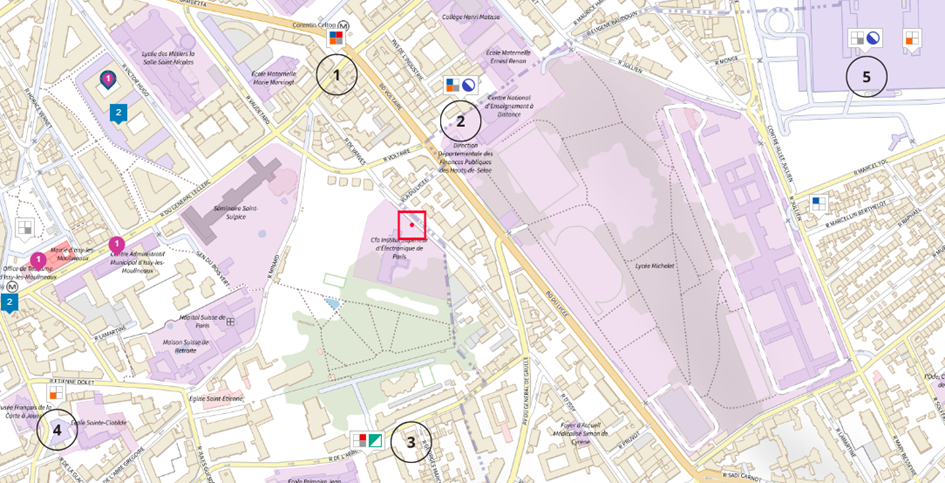
\includegraphics[width=1\linewidth]{image1.png}
    \caption{Carte des antennes proches de notre localisation}
    \label{fig:enter-label}
\end{figure}
\begin{itemize}
    \item [$\bullet$] Antenne N°1 : N° identification : 2055632 \\
    
Description du site : Intérieur sous-terrain / 0m / RATP \\

Adresse : PLACE PAUL VAILLANT COUTURIER MÉTRO CORENTIN CELTON L12 \\

Code Postal / Commune : 92130 ISSY LES MOULINEAUX \\

Téléphonie : Bouygues (3G/4G) ; Orange (3G/4G) ; SFR (2G/3G/4G) ; FREE (3G/4G) \\


    \item [$\bullet$] Antenne N°2 : N° identification : 1447454 \\
    
Description du site : Immeuble / 38m / Société HLM \\

Adresse : 35 RUE ERNEST RENAN \\

Code Postal / Commune : 92130 ISSY LES MOULINEAUX \\

Téléphonie : BOUYGUES (2G/3G/4G/5G) ; ORANGE (2G/3G/4G/5G) ; FREE (3G/4G/5G) \\

    \item [$\bullet$] Antenne N°3 : N° identification : 1903324 \\
    
Description du site : Immeuble / 23m / Société HLM \\

Adresse : 11 R DE L'ABBÉ DERRY \\

Code Postal / Commune : 92130 ISSY LES MOULINEAUX \\

Téléphonie : SFR (2G/3G/4G/5G) ; FREE (3G/4G/5G) \\

    \item [$\bullet$] Antenne N°4 : N° identification : 460465 \\
    
Description du site : Immeuble / 37m / Société HLM \\

Adresse : 13 B R AUGUSTE GERVAIS \\

Code Postal / Commune : 92130 ISSY LES MOULINEAUX \\

Téléphonie : ORANGE (2G/3G/4G/5G) \\

    \item [$\bullet$] Antenne N°5 : N° identification : 2027208 \\
    
Description du site : Bâtiment / 36m / Commune, communauté de commune \\

Adresse : 2 RUE DU 4 SEPTEMBRE \\

Code Postal / Commune : 92170 VANVES \\

Téléphonie : FREE (3G/4G/5G) \\


\end{itemize}

\subsection{Focalisation sur une antenne - Jean MANOURY}

% Question 4

Les antennes auxquelles le smartphone de l'administrateur est connecté sont équipées en technologies 2G, 3G, 4G et 5G, faisceau hertzien et BLR LTE 3500 (Technologie de transmission très haut débit sans fil en attendant le déploiement de la fibre partout).
La plupart des antennes sont installées sur des immeubles, certaines dans le métro à la station Corentin Celton. La majorité des antennes portent des infrastructures appartenant à plusieurs fournisseurs d'accès internet. 

Celle à laquelle mon téléphone est le plus vraisemblablement connecté a pour numéro d'identification 1903324. Elle est située sur le toit d'un HLM au 11 rue de l'abbé Derry, à Issy-les-Moulineaux. Elle fournit des services 2G, 3G, 4G et 5G pour SFR, et des services 3G, 4G et 5G pour Free et une antenne BLR LTE 3500 (Très haut débit sans fil).

% Question 5

On veut maintenant calculer le rayon de la zone de sécurité pour la bande de téléphonie mobile 1800Mhz.

On considère la formule du gain de l'antenne :
\begin{equation*}
    \text{G}_\text{A}(\theta)[dB] = \text{G}_\text{max}[dB] - min\left(12\left(\frac{\theta}{\theta_{3dB}}\right)^2,20\right)
\end{equation*}

Avec 
\begin{itemize}
    \item [$\bullet$] $\text{G}_{max}[dB] = 17dB$ le gain maximal de l'antenne
    \item [$\bullet$] $\theta_{3dB} = \text{\ang{70}}$ \\
\end{itemize}

Pour calculer le gain de notre antenne, il faut déterminer l'angle de notre position par rapport à l'angle d'émission de celle-ci. Pour cela, on effectue des mesures d'angle avec l'outil cartoradio (c.f. sources), comme suit : \\

On se base sur l'axe est-ouest. Par rapport à celui-ci, on mesure l'angle des antennes qui nous intéressent. On trouve pour celle qui émet vers l'ouest un angle de \ang{40} (figure~\ref{fig:antouest}) par rapport à notre axe de référence, et de \ang{21} (figure~\ref{fig:antest}) pour celle qui émet vers l'est. 

\begin{figure}[H]
    \centering
    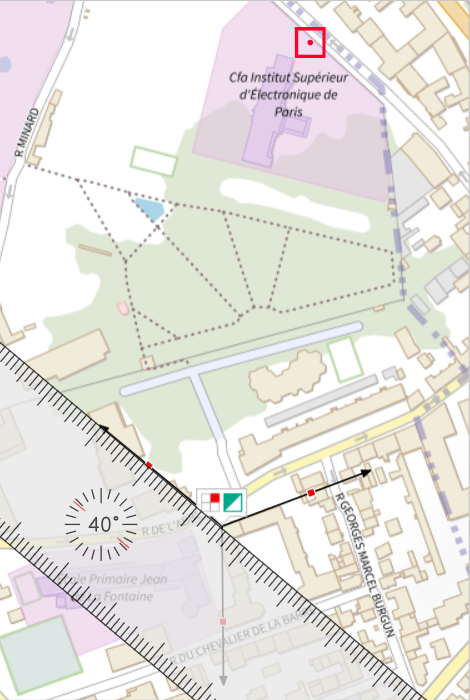
\includegraphics[width=0.3\linewidth]{antenneouest.png}
    \caption{Angle de l'antenne émettant vers l'ouest}
    \label{fig:antouest}
\end{figure}

\begin{figure}[H]
    \centering
    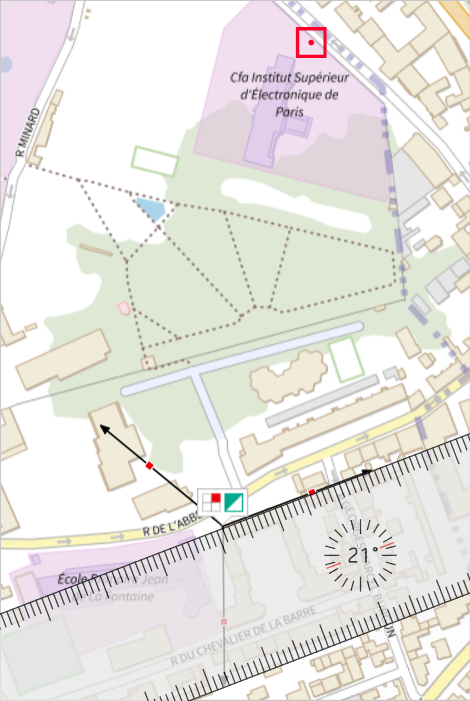
\includegraphics[width=0.3\linewidth]{antenneest.png}
    \caption{Angle de l'antenne émettant vers l'est}
    \label{fig:antest}
\end{figure}

Pour déterminer l'antenne qui assure la meilleure qualité de service selon ma position, on détermine l'angle entre ces deux antennes, puis la bissectrice de cet angle : 

\begin{equation*}
    180 - (40 + 21) = 119
\end{equation*}

\begin{equation*}
    \frac{119}{2} = \ang{59,5} \approx \ang{60}
\end{equation*}

Si on reporte cet angle sur la carte ($80 = 180 - (60 + 40)$), on peut constater que l'antenne qui assure la meilleure qualité de service est celle qui émet vers l'ouest (figure~\ref{fig:antbissec}). 

\begin{figure}[H]
    \centering
    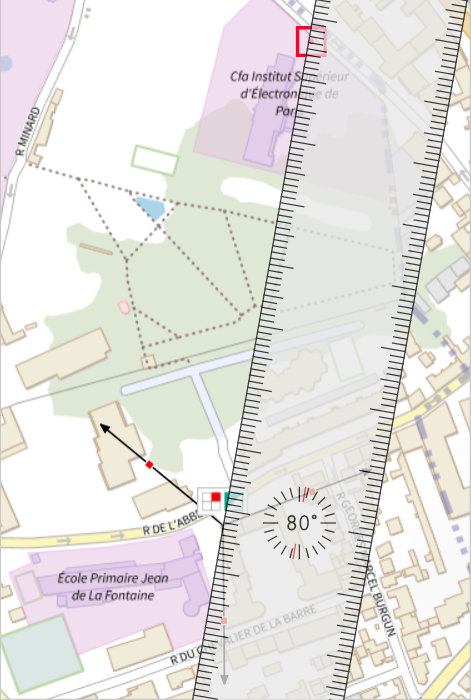
\includegraphics[width=0.3\linewidth]{bissecantennes.png}
    \caption{Bissectrice des angles des antennes}
    \label{fig:antbissec}
\end{figure}

En décalant légèrement la mesure d'angle, on trouve que ma position se trouve à \ang{81} par rapport à l'axe de référence. On trouve donc un angle de \ang{39} entre l'antenne et ma position.

Avec ces paramètres, on détermine le gain de l'antenne avec l'application numérique de la formule indiquée plus haut, en sachant que $\theta = \ang{39}$ :

\begin{equation*}
    \text{G}_\text{A}(39)[dB] = 17 - min\left(12\left(\frac{39}{70}\right)^2,20\right)
\end{equation*}

\begin{equation*}
    12 \times \left(\frac{39}{70}\right)^2 = 3,724897959 \approx 3,72
\end{equation*}

\begin{equation*}
    \text{G}_\text{A}(39)[dB] = 17 - min(3.72,20)
\end{equation*}

\begin{equation*}
    \text{G}_\text{A}(39)[dB] = 17 - 3,72 = 13,28dB
\end{equation*}

L'antenne a un gain de 13,28dB. On cherche maintenant la valeur du champ électrique de l'antenne. On prend les valeurs d'intensité du champ électrique pour les bandes de fréquence de 4G couvertes par notre antenne.

\begin{table}[H]
\centering
\resizebox{0.6\columnwidth}{!}{%
\begin{tabular}{|c|c|}
\hline
\rowcolor[HTML]{000000} 
{\color[HTML]{FFFFFF} Bande de fréquence (Mhz)} & {\color[HTML]{FFFFFF} Intensité du champ électrique (V/m)} \\ \hline
700 & 38 \\ \hline
800 & 39 \\ \hline
1800 & 59 \\ \hline
2100 & 61 \\ \hline
2600 & 61 \\ \hline
\end{tabular}%
}
\end{table}

On utilise cette relation pour mesurer le champ électrique de notre antenne :

\begin{equation*}
    \sum_{f_{i}} \left(\frac{E_{i}}{E_{l}(f_{i})}\right)^2 \leq 1
\end{equation*}

En isolant le champ électrique et en ajoutant les valeurs numériques, on trouve cette inégalité :

\begin{equation*}
    E_{i}^2\left(\frac{1}{38^2} + \frac{1}{39^2} + \frac{1}{59^2} + \frac{1}{61^2} + \frac{1}{61^2} \right) \leq 1
\end{equation*}

On sait que :

\begin{equation*}
    \text{E} = \sqrt{\frac{P_{e} G_{e} Z_{0}}{4 \pi d^2}}
\end{equation*}

On a donc : 

\begin{equation*}
    E_{i}^2 = \frac{P_{e} G_{e} Z_{0}}{4 \pi d^2} 
\end{equation*}

On prend $P_{e} \times G_{e} = 13161 W$, qu'on divise par 5 pour trouver la moyenne de la puissance d'émission sur les antennes 4G ($\frac{13161}{5} = 2632,2 W)$ et on remplace dans la formule trouvée plus haut :

\begin{equation*}
   \frac{2632,2 \times 377}{4 \pi} \left(\frac{1}{38^2} + \frac{1}{39^2} + \frac{1}{59^2} + \frac{1}{61^2} + \frac{1}{61^2}\right) \leq d^2
\end{equation*}

On peut maintenant effectuer l'application numérique pour trouver la distance de sécurité :

\begin{equation*}
    d = \sqrt{\frac{2632,2 \times 377}{4 \pi} \left(\frac{2}{61^2} + \frac{1}{38^2} + \frac{1}{39^2} + \frac{1}{59^2} \right)}
\end{equation*}

Le rayon de la zone de sécurité est $d \approx 13,10m$. \\

% Question 6

On s'intéresse maintenant à la PIRE de la station de à laquelle est connecté mon téléphone portable. On utilise comme référence une capture d'écran de l'application NetMonster (figure~\ref{fig:netmonsterpire}).

\begin{figure}[H]
    \centering
    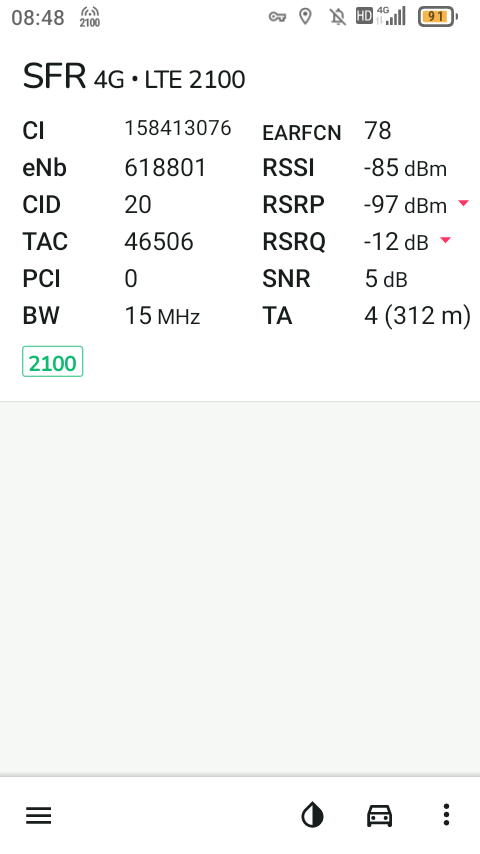
\includegraphics[width=0.3\linewidth]{screenshot_netmonster.png}
    \caption{Capture d'écran de l'application NetMonster}
    \label{fig:netmonsterpire}
\end{figure}

Tout d'abord, on va prendre comme niveau de puissance reçue une moyenne du RSSI sur quatre mesures. La fréquence porteuse du signal est 2100Mhz. Les mesures effectuées sont disponibles dans le tableau suivant :


\begin{table}[H]
\centering
\begin{tabular}{|l|l|l|l|l|}
\hline
\rowcolor[HTML]{000000} 
{\color[HTML]{FFFFFF} Mesure} & {\color[HTML]{FFFFFF} 1} & {\color[HTML]{FFFFFF} 2} & {\color[HTML]{FFFFFF} 3} & {\color[HTML]{FFFFFF} 4} \\ \hline
RSSI (dBm) & -89 & -93 & -91 & -87 \\ \hline
RSSI (W) & $1,26\times10^-12$ & $5,01\times10^-13$ & $7,94\times10^-13$ & $1,99\times10^-12$ \\
\hline
\end{tabular}
\end{table}

On trouve une moyenne de 90dBm pour le RSSI. Pour trouver la valeur de la PIRE, on utilise cette relation : PIRE [dBm] - RSSI[dBm] = Atténuation [dBm] \\

Pour trouver la puissance de transmission, on utilise la formule de l'atténuation du modèle d'Okumura-Hata :

\begin{equation*}
    A_{p} = 46,3 + 33,9 \times log_{10}(f) - 13,82 \times log_{10}(h_{b}) + (44,9 - 6,55 \times log_{10}(h_{b}) )\times log_{10}(d) - a(h_{m}) + C_{m} \\
\end{equation*}

Avec $a(h_{m})$ :

\begin{equation*}
    a(h_{m}) = 3,2 log_{10}(11,75 h_{m})^2 - 4,97
\end{equation*}

On prend comme paramètres les suivants :

\begin{itemize}
    \item $f = 2600$ : La fréquence porteuse 
    \item $h_{b} = 23m$ : La hauteur de l'antenne
    \item $h_{m} = 9m$ : La hauteur du téléphone mobile
    \item $C_{m} = 3dB$
    \item $d = 280m$ : Distance mesurée via cartoradio entre l'antenne et le mobile
\end{itemize}

On effectue l'application numérique pour trouver $a(h_{m})$ :

\begin{equation*}
    a(h_{m}) = 3,2 log_{10}(11,75 \times 9)^2 - 4,97
\end{equation*}

\begin{equation*}
    a(h_{m}) = 8.14
\end{equation*}

On effectue maintenant l'application numérique pour trouver $A_{p}$ :

\begin{equation*}
    A_{p} = 46,3 + 33,9 \times log_{10}(2600) - 13,82 \times log_{10}(23) + (44,9 - 6,55 \times log_{10}(23) )\times log_{10}(280) - 8,14 + 3
\end{equation*}

\begin{equation*}
    A_{p} = 226,16 dBm
\end{equation*}

On utilise maintenant la relation énoncée plus tôt que voici : PIRE [dBm] - RSSI[dBm] = Atténuation [dBm]

PIRE [dBm] = RSSI [dBm] + Atténuation [dBm]

En faisant l'application numérique, on trouve : 

\begin{equation*}
    \text{PIRE [dBm]} = -90 + 226,16 = 136,016
\end{equation*}

On en déduit la puissance d'émission :

\begin{equation*}
    P_{e} = PIRE - G_{A}(39)[dB] = 136,016 - 13,28 = 122,736 dBm
\end{equation*}

La puissance calculée correspond à un ressource block (RB). Pour trouver la PIRE de la station de base, il faut multiplier celle-ci par le nombre de RB correspondant à la bande passante observée. On trouve une bande passante de 15Mhz, on a donc 75 RB. En calculant, on trouve :

\begin{equation*}
    P_{e}(75) = 122,736 + 10 log_{10}(75) = 141,49 dBm 
\end{equation*}

La puissance d'émission est de 141,49 dBm.

\section{Fibre optique et câbles - Romain Oualid / Julien Chémery}

Dans le cadre de la mission que nous a fourni Events-IT, nous cherchons à relier plusieurs centres de manière filaire de la façon la plus optimisée. Nous souhaitons assurer le meilleur débit sachant que les centres se trouvent à environ 50 kilomètres l'un de l'autre. Il existe plusieurs solutions pour assurer une connexion filaire à haut débit. Dans notre cas, nous allons nous pencher sur quatre technologies distinctes : le câble coaxial, la fibre multimode à saut d'indice, la fibre multimode à gradient d'indice et la fibre monomode. 

Avant tout, nous avons comparé certaines caractéristiques de ces outils dans le tableau ci-dessous : 


\begin{table}[H]
\centering
\begin{tabular}{
>{\columncolor[HTML]{000000}}c |l|l|l|l|}
\cline{2-5}
 & \multicolumn{1}{c|}{\cellcolor[HTML]{000000}{\color[HTML]{FFFFFF} \textbf{\begin{tabular}[c]{@{}c@{}}Bande \\ passante\end{tabular}}}} & \multicolumn{1}{c|}{\cellcolor[HTML]{000000}{\color[HTML]{FFFFFF} \textbf{\begin{tabular}[c]{@{}c@{}}Puissance \\ émise\end{tabular}}}} & \multicolumn{1}{c|}{\cellcolor[HTML]{000000}{\color[HTML]{FFFFFF} \textbf{Atténuation}}} & \multicolumn{1}{c|}{\cellcolor[HTML]{000000}{\color[HTML]{FFFFFF} \textbf{Portée et débit}}} \\ \hline
\multicolumn{1}{|c|}{\cellcolor[HTML]{000000}{\color[HTML]{FFFFFF} Coaxial}} & 12 à 60 MHz& 2,3 W & 10 dB/km& \begin{tabular}[c]{@{}l@{}}Courte distance (usage \\ particulier et max 1Gb/s)\end{tabular} \\ \hline
\multicolumn{1}{|c|}{\cellcolor[HTML]{000000}{\color[HTML]{FFFFFF} Monomode}} & 1 THz (infini)& 1 à 10 W& 0,5 dB/km& \begin{tabular}[c]{@{}l@{}}Longue distance et haut débit\\ +100km\end{tabular} \\ \hline
\multicolumn{1}{|c|}{\cellcolor[HTML]{000000}{\color[HTML]{FFFFFF} \begin{tabular}[c]{@{}c@{}}Multimode\\ à saut d'indice\end{tabular}}} & 20 à 100 MHz& 1 à 10 W& 4-6 dB/km& \begin{tabular}[c]{@{}l@{}}Courte distance (quelques km\\ et vitesse réduite 8 mb/s)\end{tabular} \\ \hline
\multicolumn{1}{|c|}{\cellcolor[HTML]{000000}{\color[HTML]{FFFFFF} \begin{tabular}[c]{@{}c@{}}Multimode\\ à gradient\\ d'indice\end{tabular}}} & 2 GHz& 1 à 10 W& 3 dB/km& \begin{tabular}[c]{@{}l@{}}Moyenne distance (10 - 20 km \\ et vitesse élevé 40 - 140 Mb/s)\end{tabular} \\ \hline
\end{tabular}
\end{table}

\subsection{Caractéristiques des différents médiums - Julien Chémery}

On cherche maintenant quelle solution serait le plus adapté pour notre distance de transmission, pour ce faire on cherche d'abord la puissance reçu puis on en déduit la distance maximale d'émission pour chacun des médiums. 


\subsubsection{Cable coaxial - Julien Chémery}

\begin{equation*}
    C = B \times \log_2 \left( \text{SNR} + 1 \right)
\end{equation*}

\begin{equation*}
    \text{SNR} = 2^{\frac{C}{B}} - 1
\end{equation*}

\begin{equation*}
    \text{SNR} = 2^{ \frac{10^9}{6 \times 10^7}} -1 = 104030,9
\end{equation*}

\begin{equation*}
    \text{SNR} = \frac{RSSI}{P_e}
\end{equation*}

\begin{equation*}
    P_r = SNR \times KTB 
\end{equation*}

\begin{equation*}
    P_r = 104031 \times 1,38.10^{-23} \times 290 \times 6.10^7
\end{equation*}

\begin{equation*}
    P_r = 2,5.10^{-8} \text{ W} = -76 \text{ dBm}
\end{equation*}

On en déduit la distance maximale d'émission : 

\begin{equation*}
    d = \frac{Att}{Att_{dB/km}}
\end{equation*}

\begin{equation*}
    P_e = 2,3 \text{ W} = -26,3827 \text{ dBm}
\end{equation*}

\begin{equation*}
    Att = P_e - P_r
\end{equation*}
    
\begin{equation*}
    Att = -26,3827 - \left( -76 \right) = 49,6173 \text{ dBm}
\end{equation*}

\begin{equation*}
    d = \frac{49,6173}{10} = 4,96173 \text{ km} \approx 4,96 \text{ km}
\end{equation*}

La distance maximale d'émission du câble coaxial est donc de 4,96 km.


\subsubsection{Fibre Monomode - Julien Chémery}

Pour la fibre on a RSSI $= P_r$ car le coeficient de reflexion est nul.


\begin{equation*}
    \text{SNR} = 2^{ \frac{10^9}{10^{12}}} -1 = 0,000693
\end{equation*}

\begin{equation*}
    P_r = 0,000693 \times 1,38.10^{-23} \times 290 \times 10^{12}
\end{equation*}

\begin{equation*}
    P_r = 2,77.10^{-12} \text{ W} = -120 \text{ dBm}
\end{equation*}

On en déduit la puissance maximale d'émission : 

\begin{equation*}
    d = \frac{Att}{Att_{dB/km}}
\end{equation*}

\begin{equation*}
    P_e = 10 \text{ W} = 40 \text{ dBm}
\end{equation*}

\begin{equation*}
    Att = P_e - P_r
\end{equation*}
    
\begin{equation*}
    Att = 40 - \left( -120 \right) = 160 \text{ dBm}
\end{equation*}

\begin{equation*}
    Portée = \frac{160}{0,5} \approx 320 \text{ km}
\end{equation*}

La distance maximale d'émission d'un câble de fibre optique monomode est donc de 320 km.

\subsubsection{Fibre Multimode à saut d'indice - Julien Chémery}


\begin{equation*}
    \text{SNR} = 2^{ \frac{10^9}{10^{8}}} -1 = 1023
\end{equation*}

\begin{equation*}
    P_r = 1023 \times 1,38.10^{-23} \times 290 \times 10^{8}
\end{equation*}

\begin{equation*}
    P_r = 4,09^{-10} \text{ W} = -63,88 \text{ dBm}
\end{equation*}

On en déduit la distance maximale d'émission : 

\begin{equation*}
    d = \frac{Att}{Att_{dB/km}}
\end{equation*}

\begin{equation*}
    P_e = 10 \text{ W} = 40 \text{ dBm}
\end{equation*}

\begin{equation*}
    Att = P_e - P_r
\end{equation*}
    
\begin{equation*}
    Att = 40 - \left( -63,88 \right) = 103,88 \text{ dBm}
\end{equation*}

\begin{equation*}
    d = \frac{103,88}{6} \approx 17,31 \text{ km}
\end{equation*}

La distance maximale d'émission d'un câble de fibre optique multimode à saut d'indice est donc de 17,31 km.


\subsubsection{Fibre Multimode à gradient d'indice - Julien Chémery}


\begin{equation*}
    \text{SNR} = 2^{ \frac{10^9}{2 \times 10^{9}}} -1 = 0,414214
\end{equation*}

\begin{equation*}
    P_r = 1 \times 1,38.10^{-23} \times 290 \times 2 \times 10^{9}
\end{equation*}

\begin{equation*}
    P_r = 3,315^{-12} \text{ W} = -84,79 \text{ dBm}
\end{equation*}

On en déduit la distance maximale d'émission : 

\begin{equation*}
    d = \frac{Att}{Att_{dB/km}}
\end{equation*}

\begin{equation*}
    P_e = 10 \text{ W} = 40 \text{ dBm}
\end{equation*}

\begin{equation*}
    Att = P_e - P_r
\end{equation*}
    
\begin{equation*}
    Att = 40 - \left( -84,79 \right) = 124,79 \text{ dBm}
\end{equation*}

\begin{equation*}
    d = \frac{124,79}{3} \approx 41,598 \text{ km}
\end{equation*}

La distance maximale d'émission d'un câble de fibre optique multimode à gradient d'indice est donc de 41,598 km.

\newpage
\subsection{Comparaison et solution conseillée - Romain Oualid / Paul Morel / Julien Chémery}

\begin{figure}[H]
    \centering
    
\includegraphics[width=1\linewidth]{image.png}
    \caption{Tableau des prix des différents médiums et équipements}
    \label{fig:enter-label}
\end{figure}

\begin{table}[H]
\resizebox{\textwidth}{!}{%
\begin{tabular}{|
>{\columncolor[HTML]{000000}}c |c|c|c|c|}
\hline
\multicolumn{1}{|l|}{\cellcolor[HTML]{000000}{\color[HTML]{FFFFFF} Technologie filaire}} & \multicolumn{1}{l|}{\cellcolor[HTML]{000000}{\color[HTML]{FFFFFF} Câble coaxial}} & \multicolumn{1}{l|}{\cellcolor[HTML]{000000}{\color[HTML]{FFFFFF} Fibre optique Monomode}} & \cellcolor[HTML]{000000}{\color[HTML]{FFFFFF} \begin{tabular}[c]{@{}c@{}}Fibre optique Multimode \\ à gradient d'indice\end{tabular}} & \cellcolor[HTML]{000000}{\color[HTML]{FFFFFF} \begin{tabular}[c]{@{}c@{}}Fibre optique Multimode\\ à saut d'indice\end{tabular}} \\ \hline
{\color[HTML]{FFFFFF} Bande passante} & 12 à 60 MHz & 1 THz & 20 à 100 MHz & 2 GHz \\ \hline
{\color[HTML]{FFFFFF} Puissance reçue} & -76 dBm & -120 dBm & -63,88 dBm & -84,79 dBm \\ \hline
{\color[HTML]{FFFFFF} Distance} & 4,96 Km & 320 Km & 17,31 Km & 41,598 Km \\ \hline
{\color[HTML]{FFFFFF} Atténuation} & 10 dB/Km & 0,5 dB/Km & 4-6 dB/Km & 3 dB/Km \\ \hline
{\color[HTML]{FFFFFF} Répéteurs} & 11 & 0 & 3 & 1 \\ \hline
{\color[HTML]{FFFFFF} Prix} & 37 020 € & 503 298 € & 454 848 € & 458 048 € \\ \hline
\end{tabular}%
}
\end{table}


Après une analyse économique et pratique détaillée observable ci-dessus, nous conseillons à notre client de choisir la fibre multimode à gradient d'indice. Cette recommandation est le résultat d'une réflexion sur le rapport coût-performance. Bien que son prix soit légèrement plus élevé, la fibre multimode à gradient d'indice se distingue de la fibre multimode à saut d'indice par une meilleure bande passante, ce qui se traduit par des taux de transmission de données plus élevés. De plus, elle garantit une transmission de signal plus fiable sur de plus longues distances. En tenant compte de ces avantages, opter pour la fibre multimode à gradient d'indice constitue un investissement stratégique.

\newpage
\section*{Conclusion - Arsène Nouvellon}

En conclusion, notre analyse ainsi que nos mesures expérimentales nous ont permis de comprendre davantage les différentes technologies de communication sans fil. Nous avons comparé des technologies telles que la Wi-Fi et le Bluetooth et déterminé les avantages et les inconvénients de chacune de ces méthodes de communication. L'utilisation de l'un ou de l'autre de ces méthodes nécessite donc une évaluation minutieuse en fonction des besoins spécifiques.\\

Premièrement, le Bluetooth, il assure une communication fiable sur un périmètre réduit, il excelle donc pour l'interconnexion d'appareils personnels. Il se distingue également par sa facilité de mise en place, et sa possibilité d'interconnecter des appareils même dépourvus d'écrans ou de claviers. Toutefois, comme on a pu le voir lors de nos manipulations, il présente des limites en termes de vitesse de transfert de données, son utilisation doit donc être réfléchie et limitée à des cas spécifiques.\\

Ensuite, la Wi-Fi offre une vitesse de transmission plus élevée, même sur une grande distance. Elle est donc plus polyvalente que le Bluetooth et reste utilisable même dans le cadre de projets très coûteux en bande passante. Toutefois, il est primordial de choisir un canal cohérent afin de limiter les parasitages et les interférences et ainsi assurer une connexion stable. Sa mise en place est aussi plus complexe et plus onéreuse qu'un réseau de connexion Bluetooth.\\

Ici, nous nous concentrons principalement sur les méthodes de connexion sans fil, mais il est possible de rendre une connexion plus stable et d'en améliorer le débit en utilisant une connexion filaire. La vitesse et la stabilité de cette connexion peuvent encore être améliorées en utilisant des technologies plus récentes telles que la fibre optique, par exemple. \\

En résumé, il n'y a pas une technologie meilleure qu'une autre, chacune présente des points faibles et des points forts. Il est nécessaire de réfléchir à l'infrastructure réseau que l'on veut mettre en place et décider au cas par cas de quelle solution utiliser.\\

Dans notre cas, et pour assurer le bon fonctionnement de notre solution digitale sur les différents lieux des festivals, nous avons choisi de mélanger ces technologies. Ainsi, les administrateurs et l'équipe technique utiliseront une connexion Wi-Fi pour se connecter au serveur Web, et les différents capteurs présents sur le lieu du festival seront eux connectés en Bluetooth. Les festivaliers quant à eux seront connectés à Internet et nous feront leur retours grâce à la 4G ou la 5G. À noter que, selon la disposition et la taille des différents festivals, l'architecture de notre réseau pourrait être amenée à varier.

 

\newpage
\section*{Sources}

\begin{itemize}{\textwidth}
    \item [$\bullet$] \href{http://f5ad.free.fr/ANT-QSP_F5AD_Pertes-ROS-cable-coaxial.htm}{Câble Coaxial - Spécifications}

    \item [$\bullet$] \href{https://community.fs.com/fr/article/understanding-fiber-loss-what-is-it-and-how-to-calculate-it.html}{Understanding Fiber Loss and how to calculate it}

    \item [$\bullet$] \href{https://www.optcore.net/fr/single-mode-vs-multimode-fiber-difference/}{Fibre Monomode vs multimode, quelle différence ?}

    \item [$\bullet$]\href{https://www.thefoa.org/FR/Chapitre%205.htm#:~:text=La%20fibre%20multimode%20%C3%A0%20gradient,jusqu'%C3%A0%20environ%202%20gigahertz}{Fibre à gradient d'indice}

    \item [$\bullet$] \href{https://www.cartoradio.fr}{Carte des sites et des mesures radioélectriques en France}

    \item [$\bullet$] \href{https://www.bag.admin.ch/dam/bag/fr/dokumente/str/nis/faktenblaetter-emf/faktenblatt-bluetooth.pdf.download.pdf/faktenblatt%20bluetooth%20f.pdf}{Bluetooth Class PDF}

\end{itemize}








\end{document}